%========================================================================
\section{De la QA classique vers l'automatique}
% TIMING ~11 min  |  LE COEUR. Demarche ingenieur canonique. L'executant QA a revele le probleme.
%========================================================================

\begin{frame}{Constat de la QA pour Polène}
  \footnotesize Contexte : Polène possède un site e-commerce déployé dans plus de 20 pays. En réalité, il y a \textbf{10 sites différents} qui doivent être mis en production régulièrement.
  \vskip 8pt
  \begin{columns}[T]
    \column{.49\textwidth}
    \begin{block}{Le quotidien de la QA}
      \footnotesize
      \begin{itemize}
        \item \textbf{Homologation} : tester chaque ticket pour le valider avant la MEP
        \item \textbf{TNR} : vérifier qu'une nouvelle MEP ne casse pas les fonctionnalités déjà existantes
        \item Le tout manuellement sur un environnement de pré-prod, en lien constant avec les devs et la PO
      \end{itemize}
    \end{block}
    \column{.49\textwidth}
    \begin{alertblock}{Ce qui complique la QA sur Polène}
      \footnotesize
      \begin{itemize}
        \item Tickets \textbf{sous-spécifiés} : critères d'acceptance flous
        \item \textbf{Aucune spécification} fiable : compliqué d'avoir des points de repères pour les tests
        \item \textbf{Pas d'environnement de test} : pré-prod partagée, Golden Data manquante
      \end{itemize}
    \end{alertblock}
  \end{columns}
  \vskip 16pt
  {\footnotesize $\Rightarrow$~Impossible de réaliser les tests de manière fiable et systématique.}
\end{frame}

\begin{frame}{La première réponse et ses limites}
  \only<1>{%
      \begin{columns}[c]
      \column{.47\textwidth}\centering
        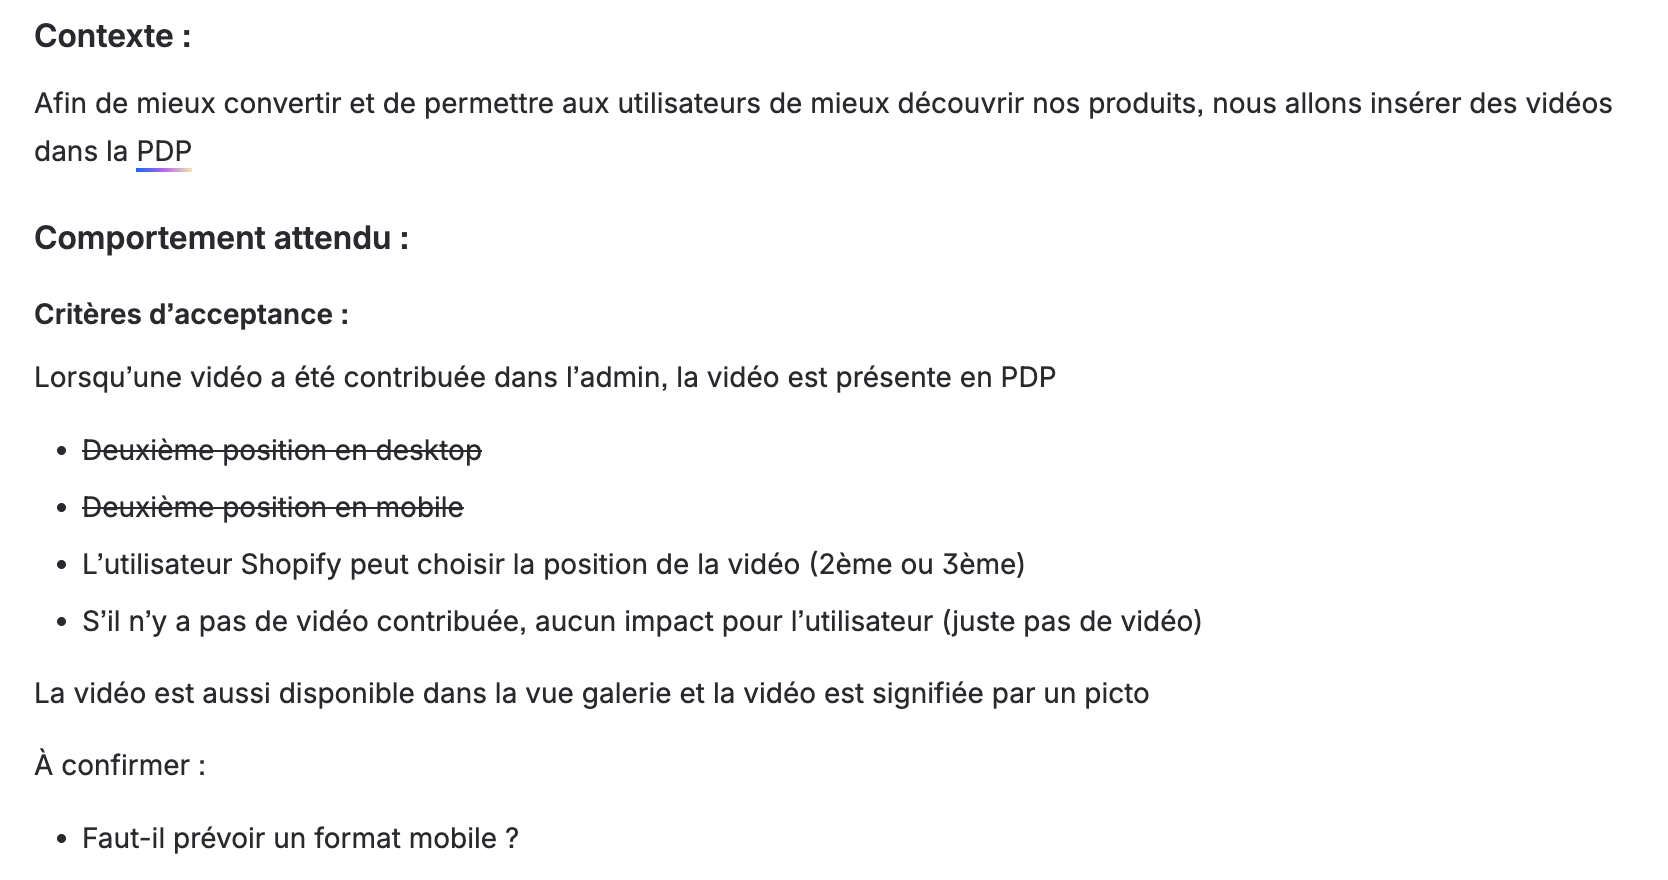
\includegraphics[width=\linewidth,height=6cm,keepaspectratio]{images/ticket}\\[2pt]
        \footnotesize Ticket initial (rédigé par la PO)
      \column{.06\textwidth}\centering $\to$
      \column{.47\textwidth}\centering
        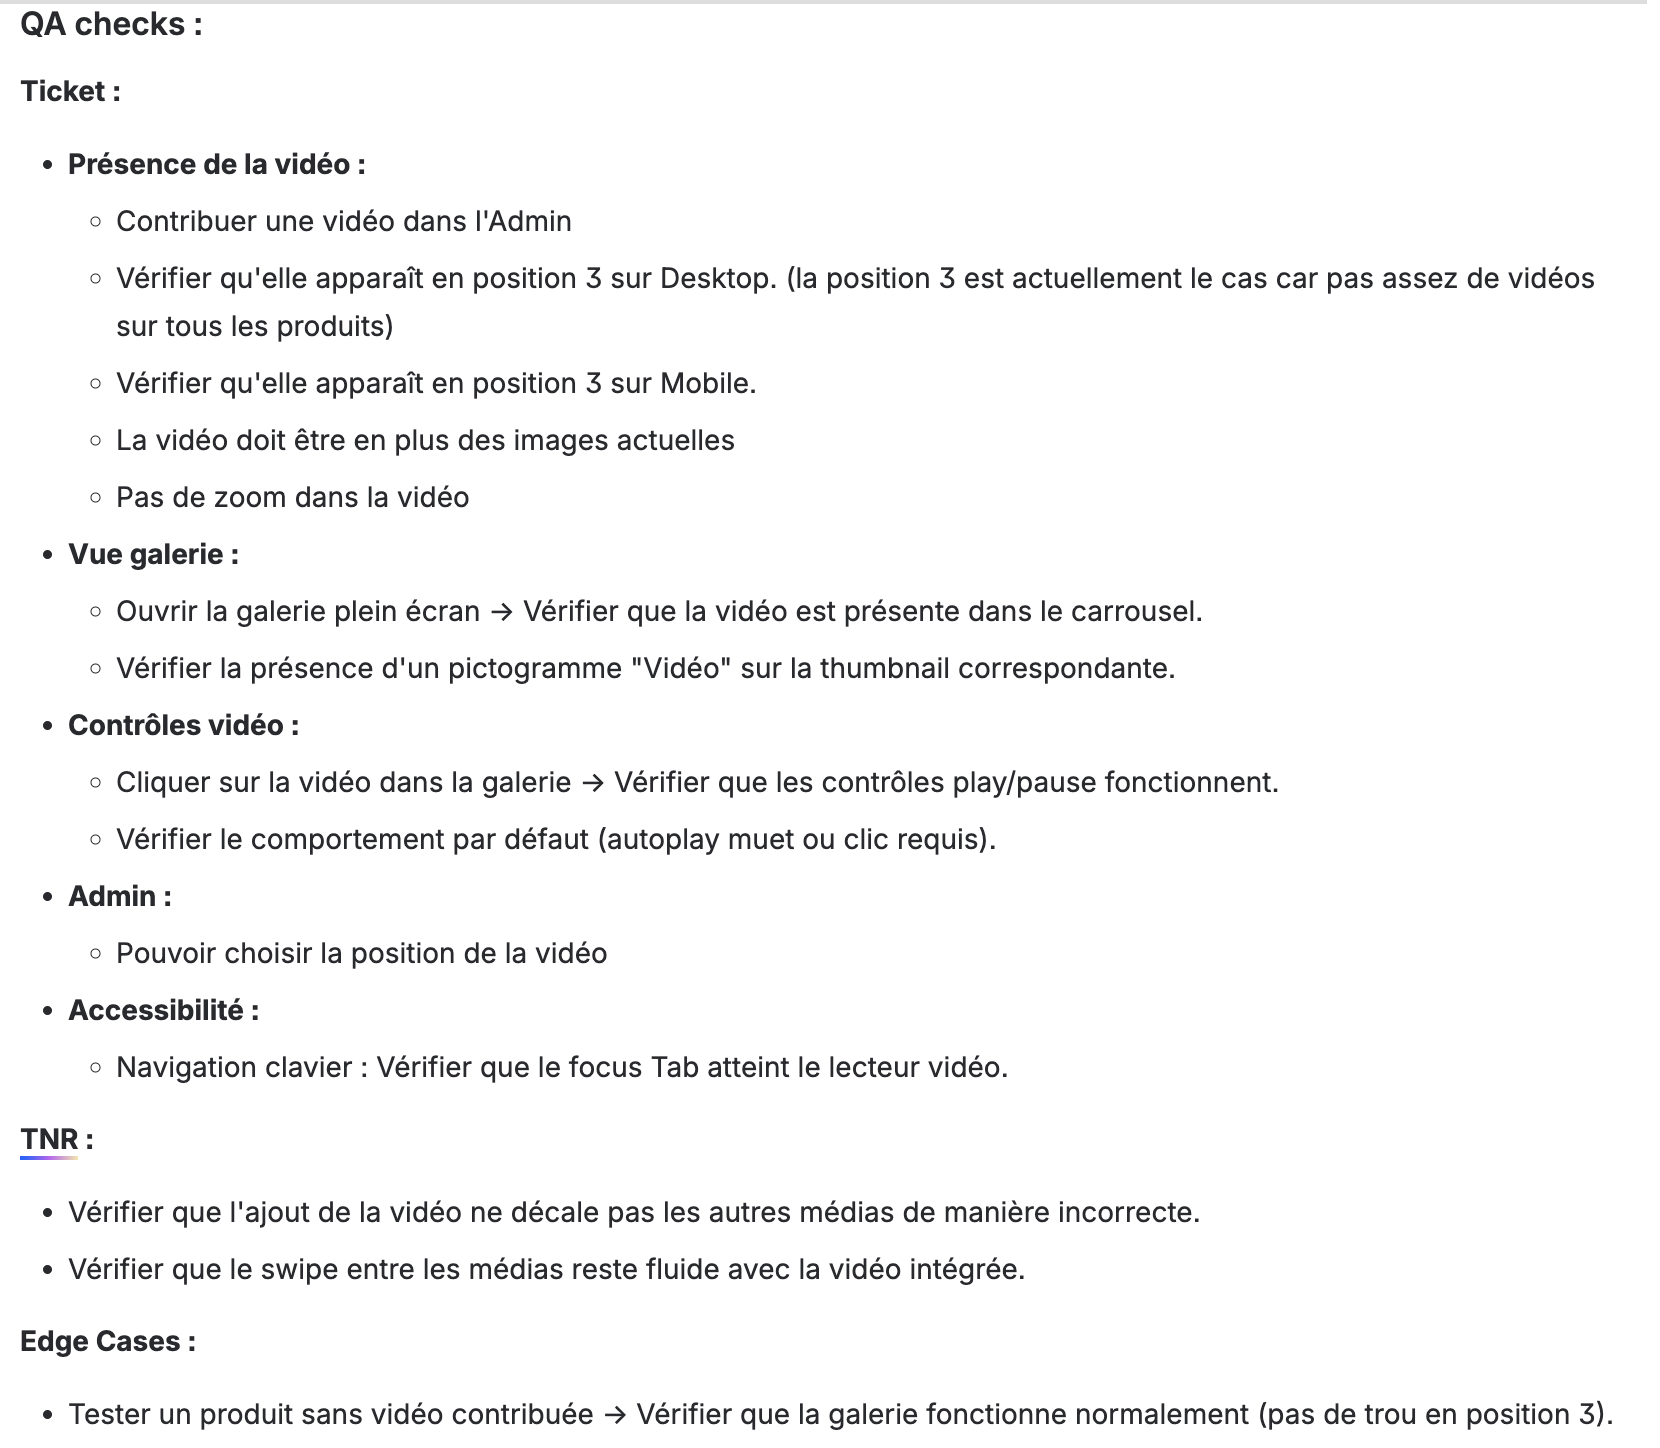
\includegraphics[width=\linewidth,height=6cm,keepaspectratio]{images/ticket_qa_checks}\\[2pt]
        \footnotesize + section "QA Checks"
    \end{columns}}
  \only<2>{%
    \begin{columns}[T]
      \column{.5\textwidth}
      \textbf{Les "QA Checks"}
      \begin{itemize}\footnotesize
        \item Section ajoutée au ticket avant le lancement des développements
        \item Palliatif aux critères d'acceptance restreints
        \item Moins d'allers-retours dev/QA/PO
      \end{itemize}
      \column{.5\textwidth}
      \textbf{Limités par construction}
      \begin{itemize}\footnotesize
        \item Vit dans le périmètre d'un ticket
        \item Aucune vision globale du site
        \item Non automatisable
      \end{itemize}
    \end{columns}}
  \only<3>{%
    \vskip 28pt
    \begin{alertblock}{Des pistes pour poursuivre le travail d'amélioration de la QA...}
      \begin{enumerate}
        \item Quelle \textbf{stratégie de documentation} des TNR adopter ?
        \item Comment exécuter des tests de manière \textbf{systématique} et \textbf{automatique} ?
      \end{enumerate}
    \end{alertblock}}
\end{frame}

\begin{frame}{Documentation des TNR}
  \footnotesize \textbf{Objectif} : pour chaque page du site, documenter les TNR, c'est-à-dire la liste essentielle de chaque élément à vérifier avant les MEP.
  \vskip 8pt
  \begin{alertblock}{Le vrai enjeu : à quel niveau de détail documenter ?}
    \footnotesize
    \begin{itemize}
      \item \textbf{Trop fin} : la page d'accueil documentait 28 éléments différents \\$\to$ pour un seul QA sur Polène c'est trop compliqué à maintenir
      \item \textbf{Trop vague} : des éléments vont être oubliés lors des tests
    \end{itemize}
  \end{alertblock}
  \vskip 2pt
  \begin{exampleblock}{Mon choix : documenter par blocs cohérents}
    \begin{itemize}
      \item Chaque \textbf{composant Shopify} = un élément à documenter
      \item Niveau trouvé par expérimentation sur la page d'accueil
      \item Ce niveau reste maintenable pour un dispositif comme Polène
    \end{itemize}
  \end{exampleblock}
\end{frame}

\begin{frame}[plain]
  % VOIX ~30 s. Illustration concrete des 3 niveaux de granularite sur la PLP Cyme.
  \centering
  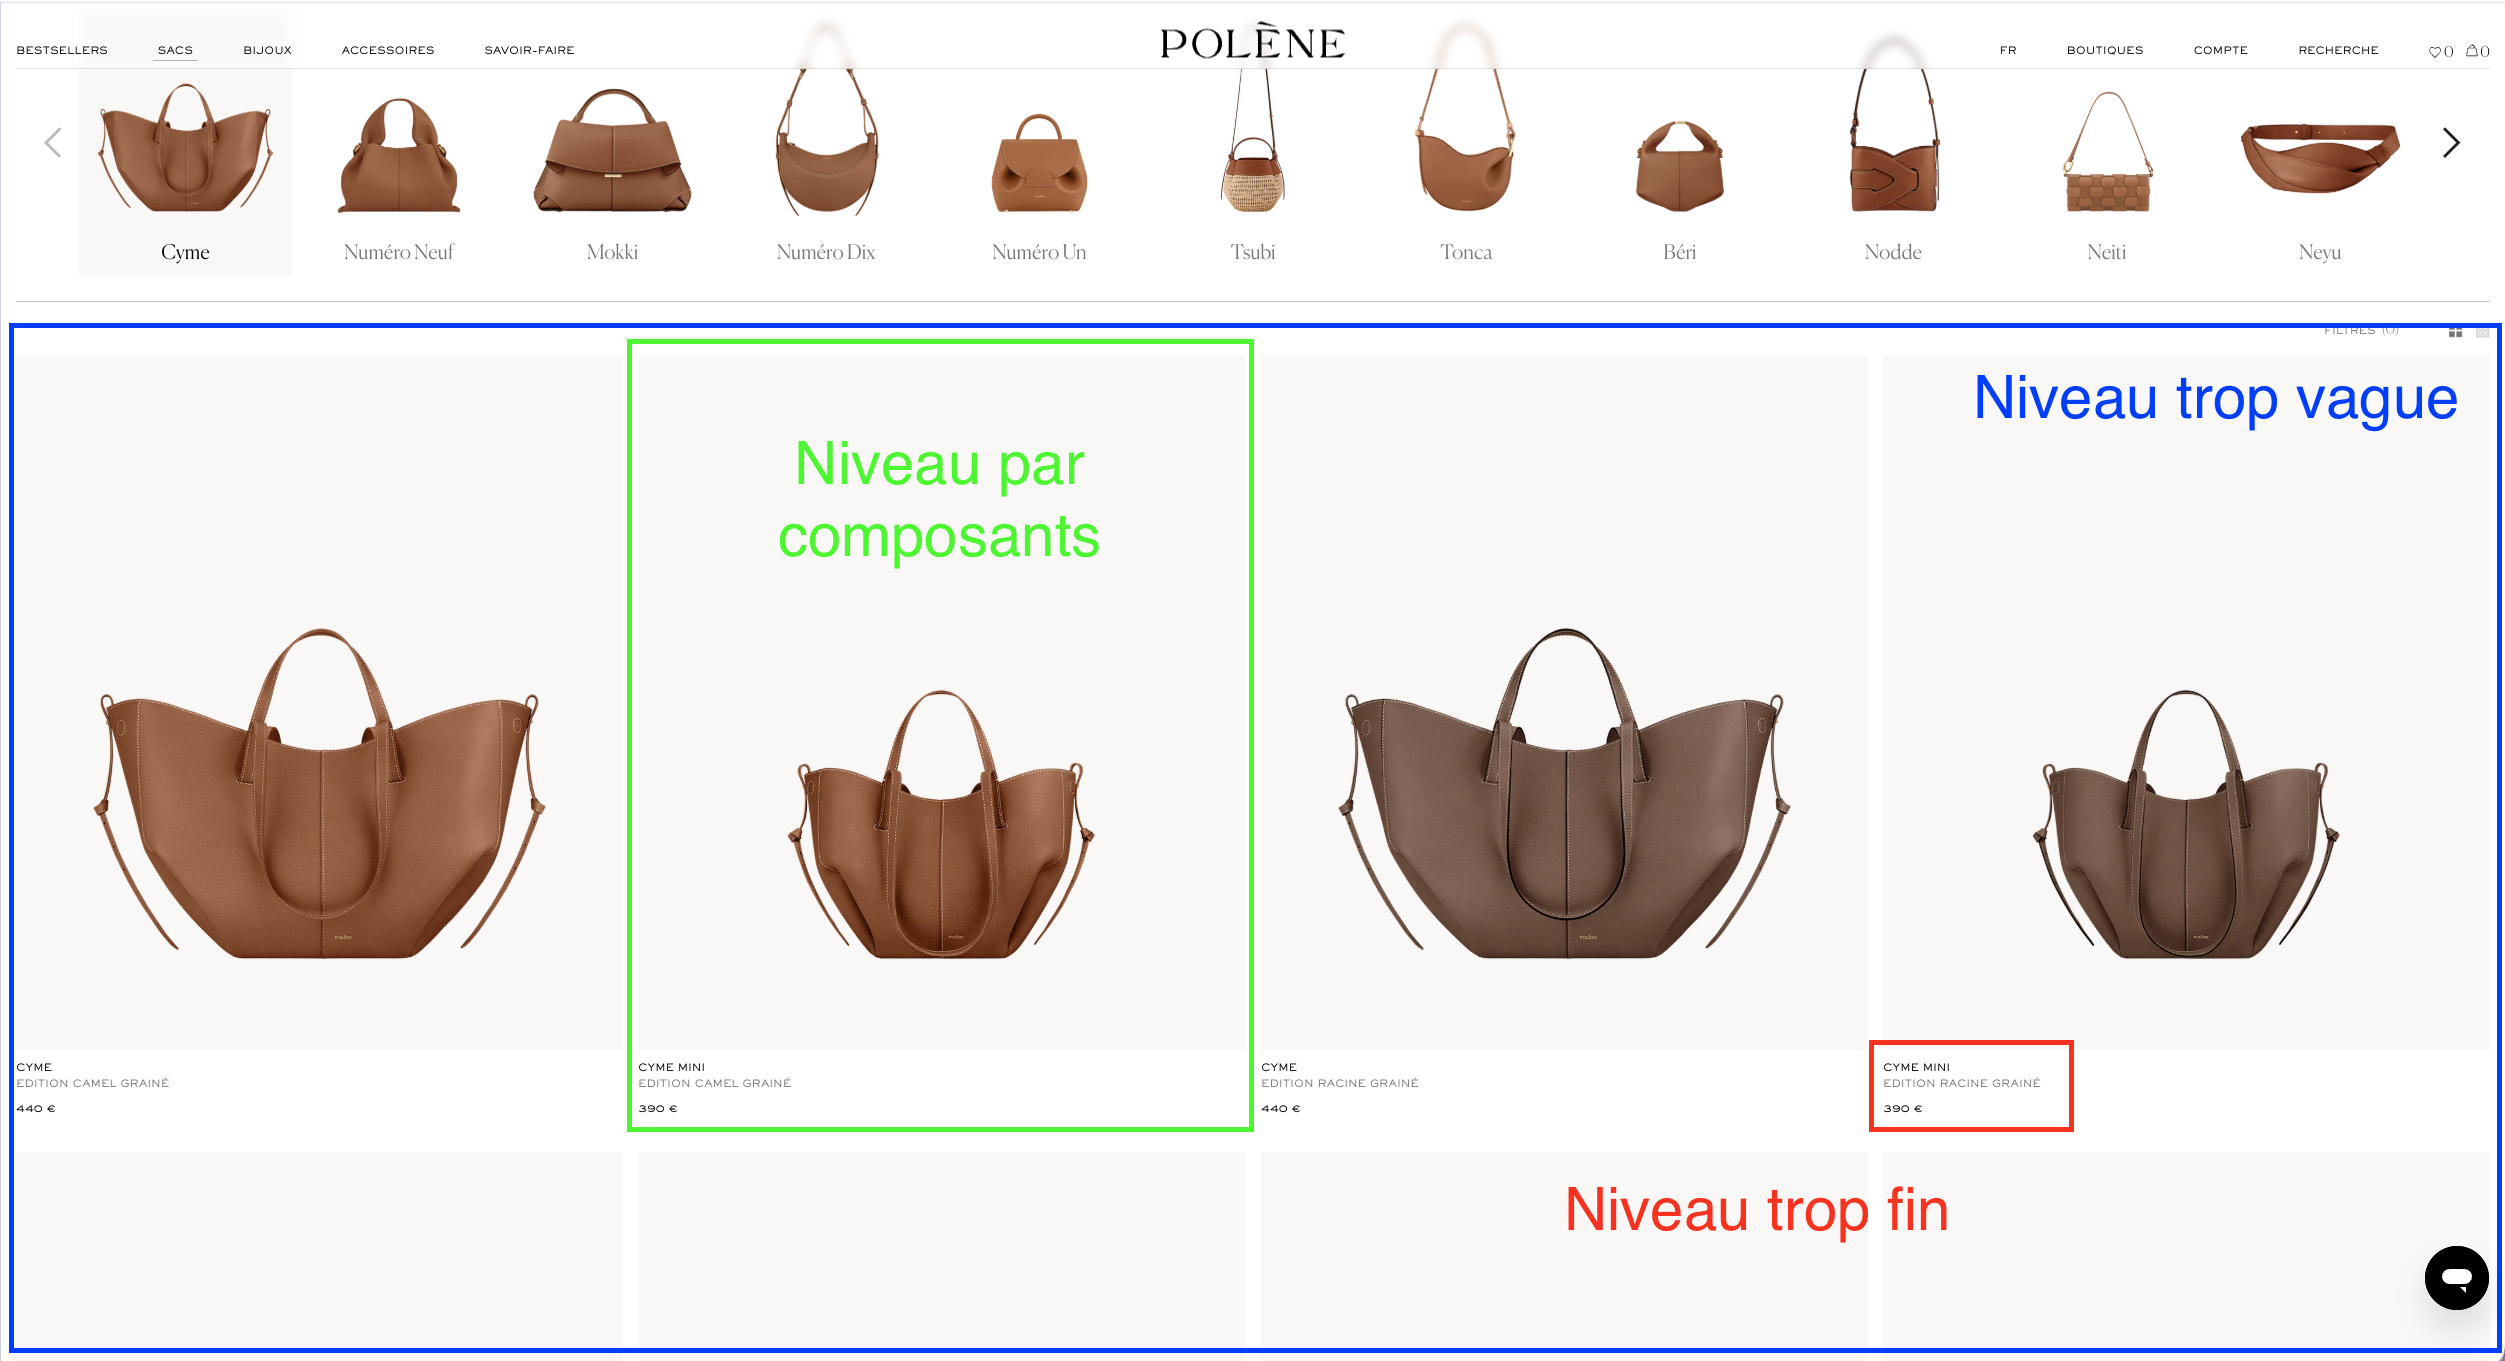
\includegraphics[height=0.9\paperheight,width=\paperwidth,keepaspectratio]{images/granularite_tnr}\\[3pt]
  {\scriptsize Trois niveaux d'abstraction pour la documentation sur la PLP}
\end{frame}

\begin{frame}{Documenter par blocs : avant / après}
  \only<1>{
    \centering 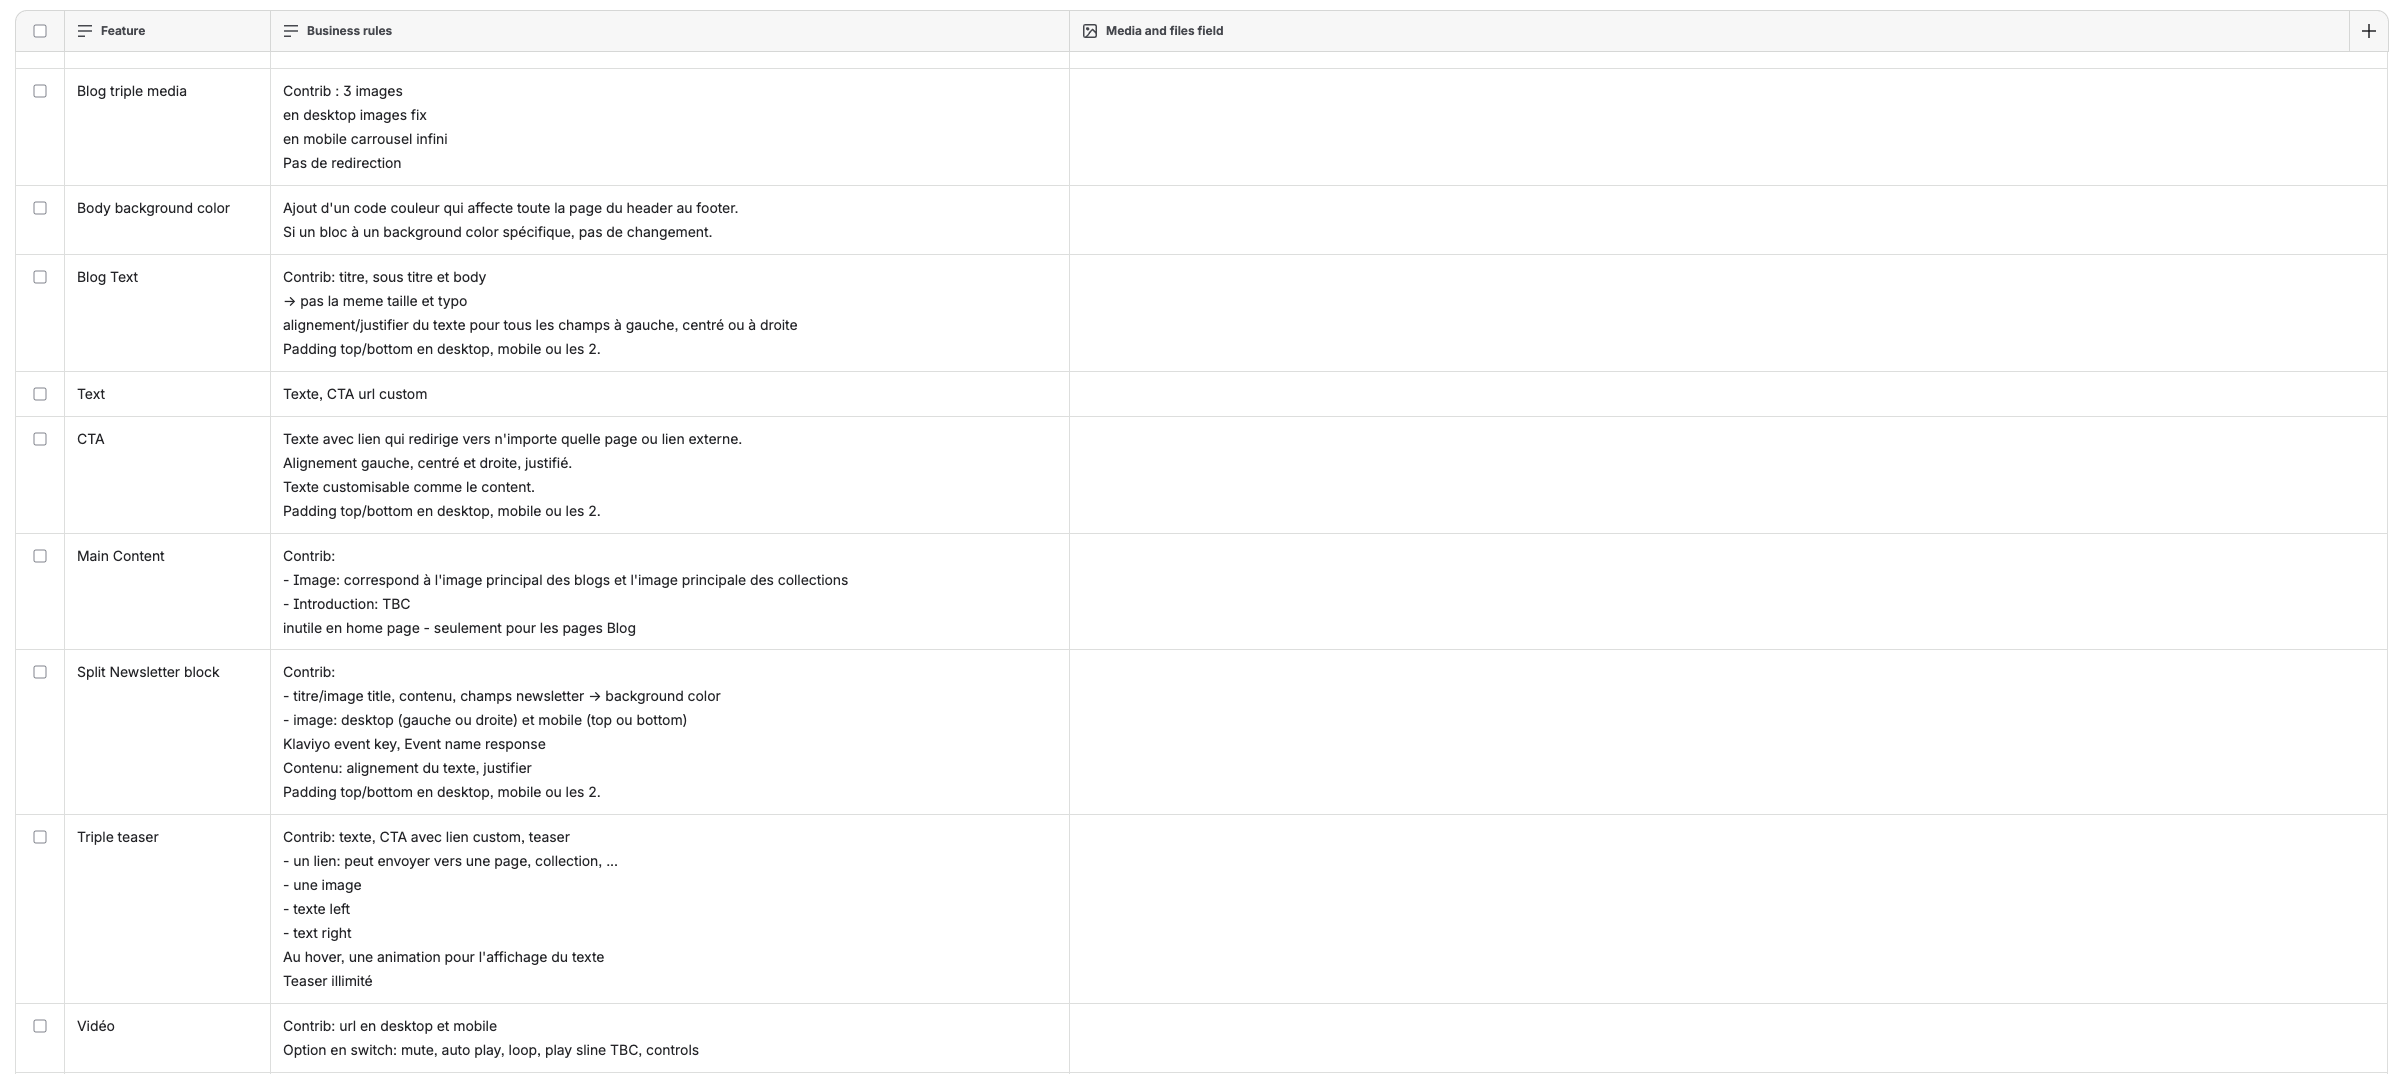
\includegraphics[width=\linewidth,height=6cm,keepaspectratio]{images/old_page_confluence}\\[4pt]
    \centering \textbf{Avant} : tableau non trié avec des informations inexploitables}
  \only<2>{
    \centering 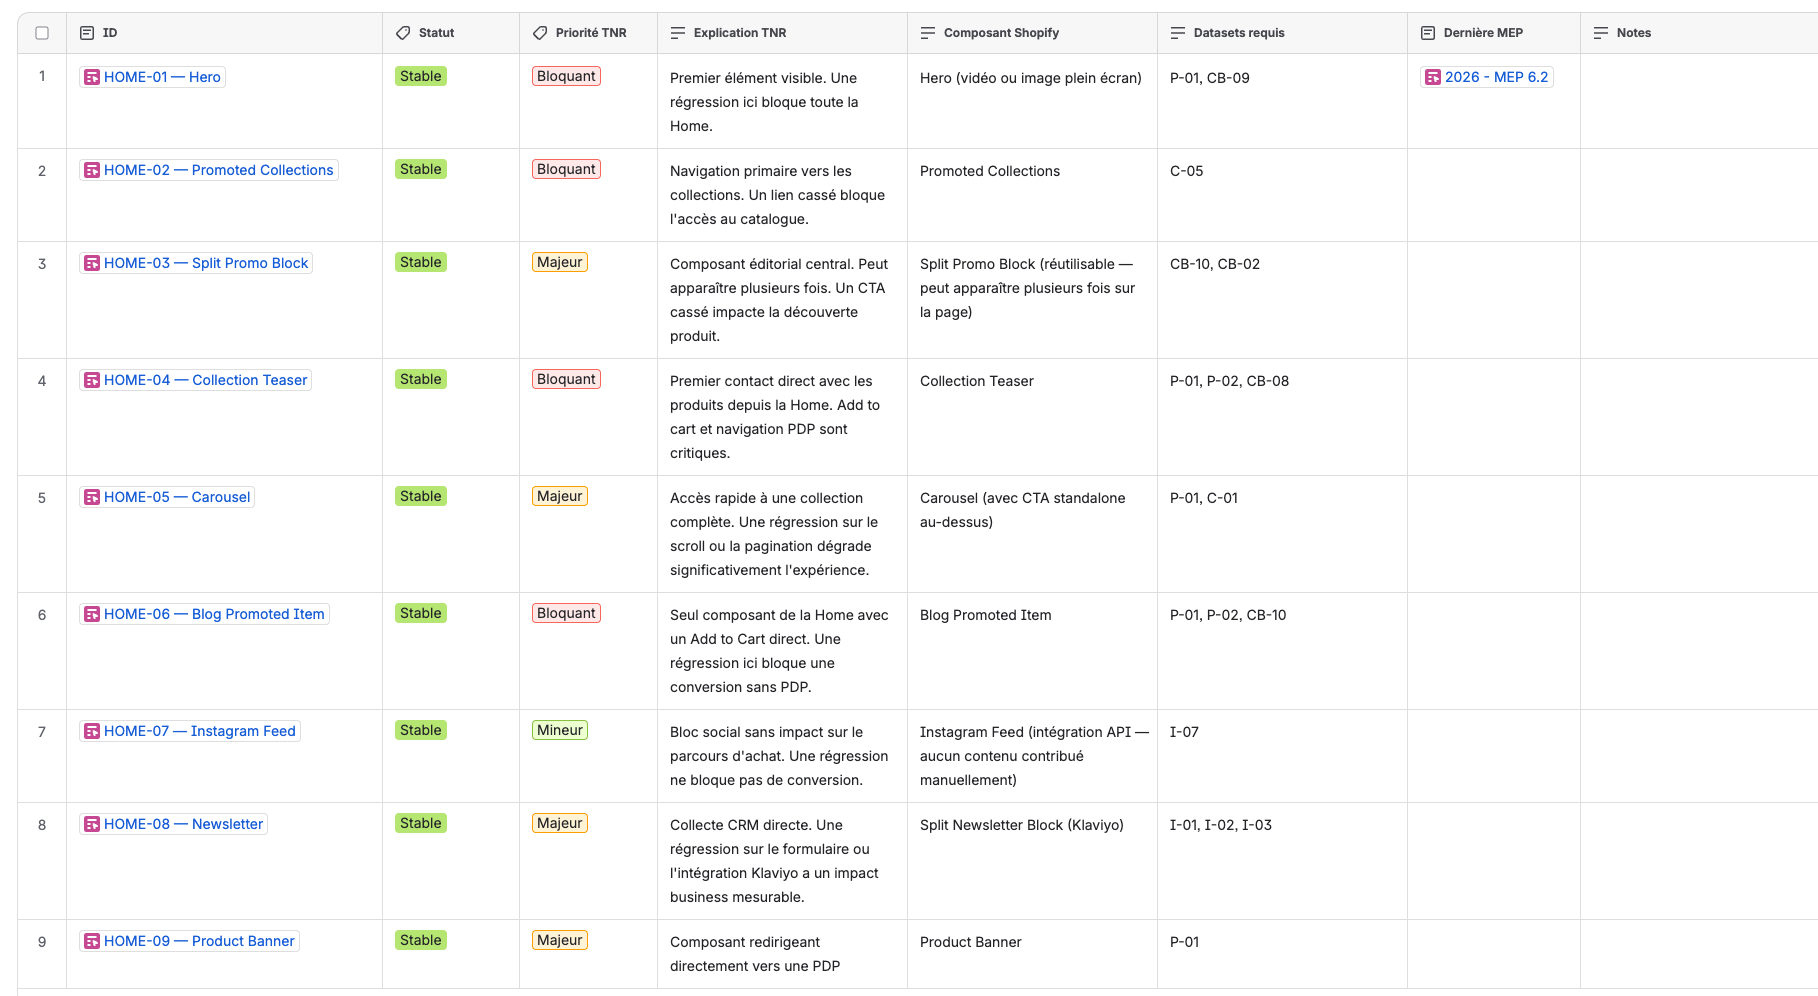
\includegraphics[width=\linewidth,height=6cm,keepaspectratio]{images/new_doc_confluence}\\[4pt]
    \centering \textbf{Après} : tableau trié avec des informations utilisables}
\end{frame}

\begin{frame}{Construction de la documentation}
  \centering
  \resizebox{\textwidth}{!}{%
  \begin{tikzpicture}[
      node distance=0.6cm, font=\footnotesize,
      skill/.style={rectangle, rounded corners=3pt, draw=ClaudeOrange, thick,
          fill=ClaudeOrange!12, text width=2.6cm, align=center,
          text=ClaudeDark, minimum height=0.9cm, inner sep=3pt},
      data/.style={rectangle, draw=GRIS, thick, fill=GRIS!6,
          text width=2.4cm, align=center, minimum height=0.9cm, inner sep=3pt},
      io/.style={rectangle, rounded corners=8pt, draw=GRIS!80!black, very thick,
          fill=white, text width=2.2cm, align=center, minimum height=0.9cm, inner sep=3pt},
      output/.style={rectangle, rounded corners=3pt, draw=ClaudeDark, thick,
          fill=ClaudeCream, text width=2.6cm, align=center, minimum height=0.9cm, inner sep=3pt},
      arr/.style={-{Stealth[length=2mm]}, thick, draw=GRIS!90!black}
  ]
    \node[io] (site) {Site de prod Polène};
    \node[skill, right=of site] (mapper) {\texttt{site-mapper}};
    \node[data, right=of mapper] (mdraw) {Markdown exhaustif};
    \node[skill, right=of mdraw] (tnr) {\texttt{site-mapper-}\\\texttt{to-tnr}};
    \node[data, right=of tnr] (mdtnr) {Markdown TNR};
    \draw[arr] (site) -- (mapper);
    \draw[arr] (mapper) -- (mdraw);
    \draw[arr] (mdraw) -- (tnr);
    \draw[arr] (tnr) -- (mdtnr);
    \node[skill, above right=0.5cm and 0.8cm of mdtnr] (conf) {\texttt{tnr-to-}\\\texttt{confluence}};
    \node[data, right=of conf] (confdoc) {Documentation Confluence (DOCX + CSV)};
    \node[skill, below right=0.5cm and 0.8cm of mdtnr] (prompt) {\texttt{tnr-to-prompt}};
    \node[data, right=of prompt] (rapport) {Prompt pour Antigravity};
    \draw[arr] (mdtnr.east) -- ++(0.4,0) |- (conf.west);
    \draw[arr] (mdtnr.east) -- ++(0.4,0) |- (prompt.west);
    \draw[arr] (conf) -- (confdoc);
    \draw[arr] (prompt) -- (rapport);
    \node[below=0.15cm of mapper, text=ClaudeDark, font=\scriptsize\bfseries] {Production de la documentation};
    \node[below=0.15cm of tnr, text=ClaudeDark, font=\scriptsize\bfseries] {Réduction en composants};
    \node[below=0.15cm of conf, text=ClaudeDark, font=\scriptsize\bfseries] {Exploitation documentation};
    \node[below=0.15cm of prompt, text=ClaudeDark, font=\scriptsize\bfseries] {Exploitation outil QA};
  \end{tikzpicture}%
  }
  \centering Pipeline de skills Claude
  \vskip 10pt
  \begin{block}{Fonctionnement du pipeline}
    \footnotesize
    \begin{itemize}
      \item \textbf{Quatre skills séparées} : générique et réapplicable à d'autres sites en adaptant l'entrée
      \item \textbf{Rétro-spec} : faute de spécification, on reconstruit depuis la production \\$\to$ limite connue : un bug en production peut devenir une norme
    \end{itemize}
  \end{block}
\end{frame}

\begin{frame}{Comment exécuter les tests documentés ?}
  \footnotesize Deux familles : des \textbf{outils dédiés} (BrowserStack, Mr Suricate, \dots) où l'on code des scénarios, ou l'\textbf{exploration autonome par IA} (Claude + Chrome, Antigravity, \dots) où un agent les déduit de la documentation.
  \vskip 4pt
  \scriptsize
  \begin{center}
  \begin{tabular}{lll}
    \toprule
    \textbf{Critère} & \textbf{Outil dédié} & \textbf{Exploration IA} \\
    \midrule
    Mise en place   & Élevé (1 j/scénario)     & Modéré (1 prompt) \\
    Maintenance     & Élevée (casse souvent)   & Faible (doc générée) \\
    Réutilisabilité & Limitée                  & Élevée \\
    Déterminisme    & Élevé                    & Modéré (variabilité liée aux LLM) \\
    Vérifiabilité   & Directe (assertions)     & Indirecte (rapport) \\
    \bottomrule
  \end{tabular}
  \end{center}
  \vskip 2pt
  \begin{block}{Choix : Exploration IA via Antigravity}
    \footnotesize Critère décisif : le \textbf{coût de maintenance}. \\Les outils dédiés à la QA ont du mal à réparer les scénarios de tests en cas de changement de contenu (produit retiré, bannière remplacée), ce qui bouge le plus sur Polène.
  \end{block}
\end{frame}

\begin{frame}{Antigravity : explorer le site comme un "humain"}
  \footnotesize \textbf{Google Antigravity} : un IDE natif IA doté d'un sous-agent navigateur piloté par le modèle de vision Gemini 3 Pro.
  \vskip 6pt
  \begin{columns}[T]
    \column{.5\textwidth}
    \begin{block}{Comment ça marche ?}
      \footnotesize
      \begin{enumerate}
        \item Un \textbf{prompt} dérivé de la documentation TNR décrit les éléments à vérifier (tnr-to-prompt)
        \item Le sous-agent \textbf{explore} le site et capture le rendu
        \item Il produit un \textbf{rapport vérifiable} (captures + vidéos)
      \end{enumerate}
      Aucun scénario codé : l'agent les déduit du prompt
    \end{block}
    \column{.46\textwidth}
    \begin{exampleblock}{Pourquoi Gemini pour la vision ?}
      \begin{itemize}
        \item \textbf{Meilleur modèle} de vision en mars \textit{(classement LMArena)} \\$\to$ Analyse le rendu visuel du site, pas seulement le DOM
      \end{itemize}
    \end{exampleblock}
  \end{columns}
\end{frame}

\begin{frame}{Antigravity : la phase d'exploration}
  \centering
  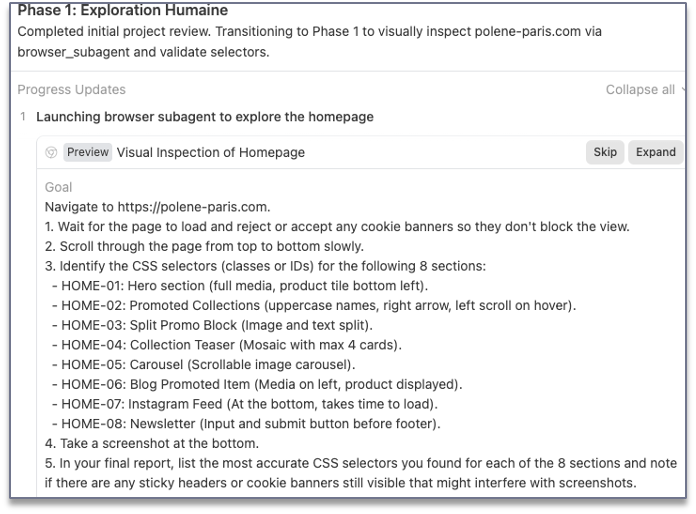
\includegraphics[width=\linewidth,height=6.7cm,keepaspectratio]{images/antigravity_execution_1}\\[4pt]
  \textbf{Phase 1} : le sous-agent explore le rendu des composants
\end{frame}

\begin{frame}{L'obstacle du coût d'exécution}
  \begin{alertblock}{Le problème}
    \begin{itemize}
      \item L'agent natif d'Antigravity réalisait \textbf{l'exploration visuelle} et \textbf{les captures d'écran}
      \item Les premiers tests ont montré \textbf{$\sim$1h} pour la page d'accueil (9 fonctionnalités à tester)
    \end{itemize}
  \end{alertblock}
  \vskip 8pt
  \begin{exampleblock}{La ré-architecture du prompt}
    \footnotesize Séparer les rôles :
    \begin{itemize}
      \item Le sous-agent explore une fois le site (vérification du rendu visuel, comportement des composants) et repère les balises HTML des composants \textbf{(Phase 1)}
      \item Puis délègue les captures d'écrans à Playwright avec les balises déjà identifiées \textbf{(Phase 2)} \\Résultat : $\sim$20 min par page
    \end{itemize}
  \end{exampleblock}
\end{frame}

\begin{frame}{Playwright fait les captures}
  \centering
  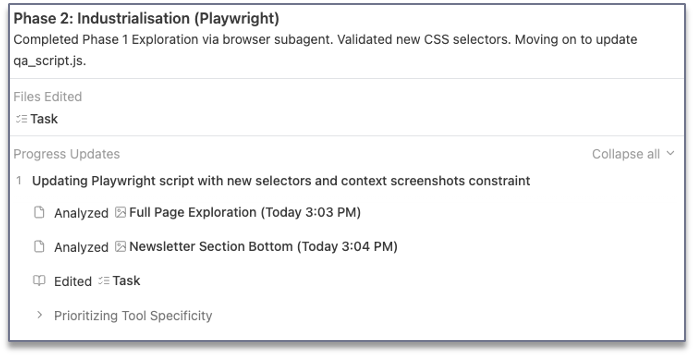
\includegraphics[width=\linewidth,height=6cm,keepaspectratio]{images/antigravity_execution_2}\\[4pt]
  \textbf{Phase 2} : Playwright réalise les captures à partir des balises identifiées
\end{frame}

\begin{frame}{Un rapport vérifiable}
  \only<1>{
    \centering 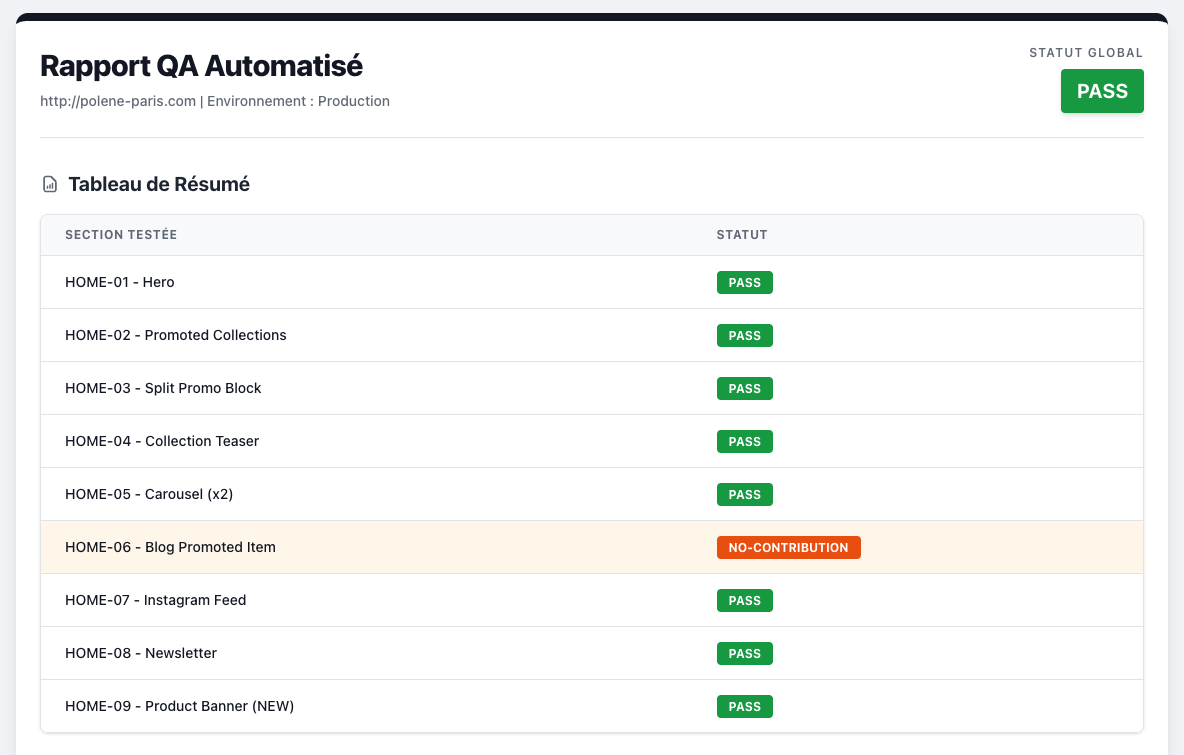
\includegraphics[width=\linewidth,height=6.7cm,keepaspectratio]{images/rapport_qa_1}\\[2pt]
    \centering \textbf{Phase 3} : Génération du rapport}
  \only<2>{
    \centering 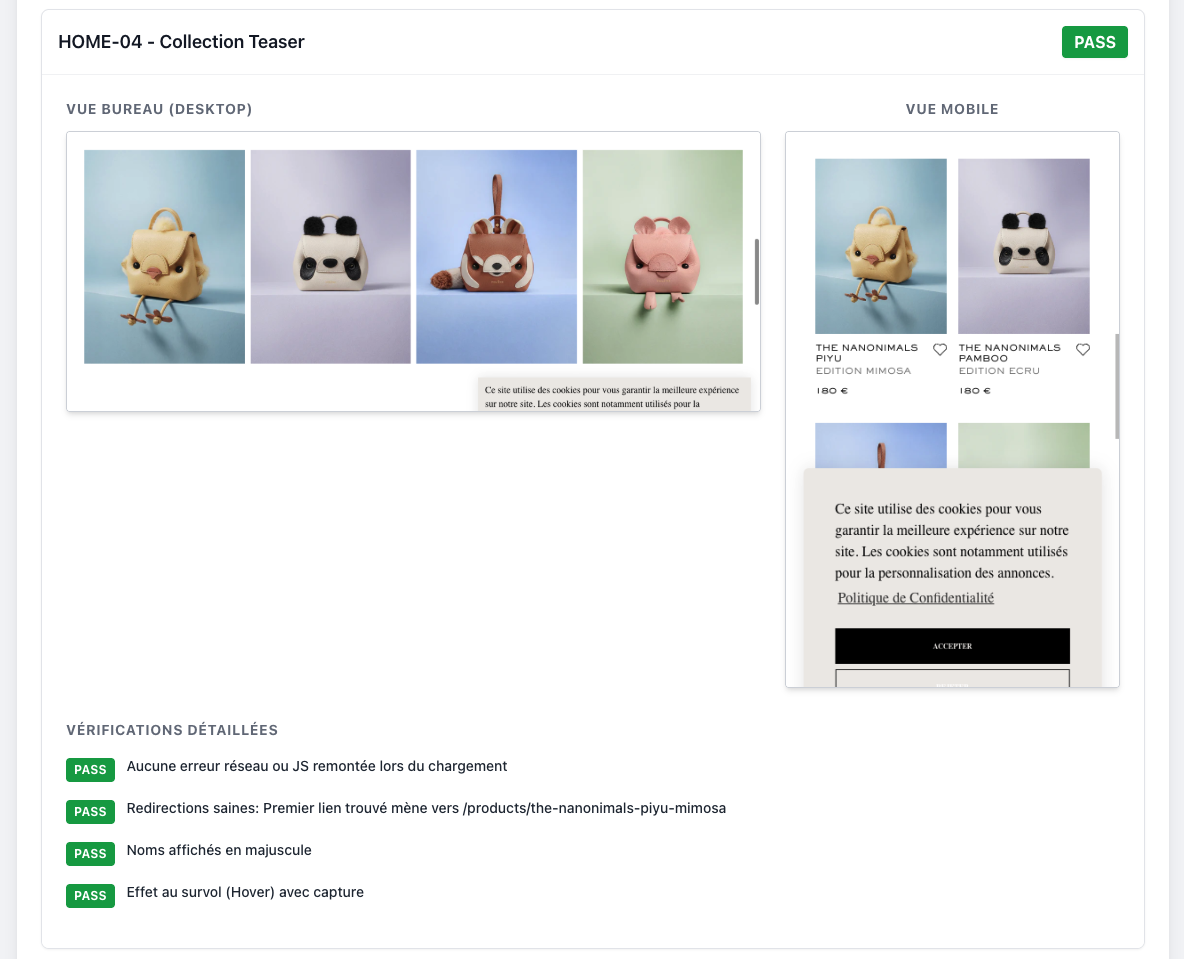
\includegraphics[width=\linewidth,height=7cm,keepaspectratio]{images/rapport_qa_2}\\[4pt]
    \centering \textbf{Pour chaque composant} : rendu desktop / mobile + vérifications}
\end{frame}

\begin{frame}{Résultats et limites}
  \begin{exampleblock}{Ce qui a été construit}
    \begin{itemize}
      \item Une chaîne de documentation et d'exécution de tests reproductible sur d'autres sites e-commerce similaires
      \item Les \textbf{6 pages principales} du site sont documentées et exécutables avec Antigravity (Accueil, PLP, PDP, Compte client, Panier, Checkout)
    \end{itemize}
  \end{exampleblock}
  \vskip 1pt
  \begin{columns}[T]
    \column{.45\textwidth}
    \begin{alertblock}{Limites assumées}
      \footnotesize
      \begin{itemize}
        \item Environnement pré-prod non maîtrisé
        \item Variations liées aux LLM
        \item Chrome desktop/mobile
      \end{itemize}
    \end{alertblock}
    \column{.5\textwidth}
    \begin{block}{Pour aller plus loin}
      \footnotesize
      \begin{itemize}
        \item Environnement de test dédié (Golden Data)
        \item Couverture Safari/mobile
        \item Intégrer en CI/CD
      \end{itemize}
    \end{block}
  \end{columns}
  \vskip 16pt
  {\footnotesize $\Rightarrow$~À retenir : démarche dans l'utilisation de l'IA (niveau d'abstraction, architecture, coût allégé de 1h à 20min)}
\end{frame}
